\documentclass{article}
\usepackage{graphicx}
\usepackage[a4paper, left=2cm, right=2cm, top=2.5cm, bottom=2cm]{geometry}
\usepackage[small]{titlesec}
\usepackage{subcaption} 
\usepackage[italian]{babel}
\usepackage[hidelinks]{hyperref}
\usepackage{listings}
\usepackage{sectsty}
%\usepackage[light]{CormorantGaramond}
\usepackage{fancyhdr}
\usepackage{footnote}
\usepackage{tgadventor}
\usepackage{titling}
\usepackage{graphicx}
\usepackage{tcolorbox}
\usepackage{multirow}
\usepackage{booktabs}
\usepackage{makecell}

\setlength{\droptitle}{-5em}   % regola la posizione del titolo
\pretitle{\begin{center}\LARGE}   % imposta la dimensione della font del titolo
\posttitle{\end{center}}
%\lstset{language=C}
\renewcommand\bfdefault{bx}
\sectionfont{\fontsize{20.74}{15}\selectfont}
\subsectionfont{\fontsize{17.28}{15}\selectfont}
\subsubsectionfont{\fontsize{12}{15}\selectfont}
\title{}

\author{}
\date{\today}


\begin{document}
\pagestyle{fancy}
\fancyhf{}
%\rhead{\thepage}
%\lhead{\rightmark}
\rfoot{\thepage}
\lhead{\quad \leftmark}
\rhead{ \quad \rightmark}

\renewcommand{\headrulewidth}{0.2pt}



\begin{titlepage}
    \begin{figure}[t]
        \centering
        
\includegraphics[width=0.7\textwidth]{im/logo_sapienza_new.png}
        \label{fig:logo}
    \end{figure}    
    \null\vfill
    \begin{center}
      {\Huge Appunti di Basi Dati Modulo I} \\[2cm]
      {\Large Colacel Alexandru Andrei}
    \end{center}
    \vfill\null
    \renewcommand{\abstractname}{Disclaimer}

    
    
    \begin{abstract}  
    
    \hrulefill


    Le fonti sono le Hand Notes del prof tradotte in italiano con l'obiettivo di migliorare la leggibilità.\\
    \textbf{Nota: è vietata assolutamente la vendita di questo materiale in qualsiasi forma senza il mio consenso.}  

    
    \hrulefill

    \end{abstract}
  \end{titlepage}


\pagebreak
\tableofcontents

\pagebreak


\section{Lemma della Chiusura}
Sia $R$ uno schema e sia $F$ un insieme di dipendenze funzionali definite su $R$. Si ha che:\par 
\begin{equation}
X \rightarrow Y \in F^{A} \Longleftrightarrow Y \subseteq X^{+}
\end{equation}

\subsection{Dimostrazione $\Rightarrow$}

Dato $X$ $\rightarrow$ $Y \in F^{A}$, per la regola della decomposizione, otteniamo:
\begin{equation}
X \rightarrow A \in F^{A}, \quad \forall A \in Y  
\end{equation} 
e quindi, per definizione di $X^{+}$, otteniamo che: 
\begin{equation}
A \in X^{+}, \quad \forall A \in Y  
\end{equation}
che significa: 
\begin{equation}
Y \subseteq X^{+}
\end{equation}


\subsection{Dimostrazione $\Leftarrow$}
Dato: 
\begin{equation}
Y \subseteq X^{+}
\end{equation}
si ottiene che: 
\begin{equation}
X \rightarrow A \in F^{A} \quad \forall A \in Y
\end{equation}
che implica, per la regola dell'unione, che: 
\begin{equation}
X \rightarrow Y \in F^{A}
\end{equation}

\pagebreak
\section{Teorema $F^{+}$ = $F^{A}$}

Dato uno schema $R$ e un insieme $F$ di dipendenze funzionali definite su $R$, si ha che:
\begin{equation}
  F^{+} = F^{A}
\end{equation}

\subsection{Dimostrazione $F^{A} \subseteq F^{+}$}
\begin{itemize}
  \item \textbf{Caso base} (n = 0): se $X \rightarrow Y \in F^{A}$ senza aver applicato alcun assioma di Armstrong, allora l'unica possibilità è che:
  \begin{equation}
    X \rightarrow Y \in F^{A} \Leftrightarrow X \rightarrow Y \in F
  \end{equation}
  Siccome $X \rightarrow Y \in F$, allora 
  \begin{equation}
    X \rightarrow Y \in F \Rightarrow X \rightarrow Y \in F^{+}
  \end{equation} 
  \item \textbf{Ipotesi induttiva forte:} ogni dipendenza funzionale in $F^{A}$ ottenuta da $F$
  applicando k $\leq$ n assiomi di Armstrong è anche in $F^{+}$:
  \begin{equation}
    X \rightarrow Y \in F^{A} tramite k \leq n assiomi \Rightarrow X \rightarrow Y \in F^{+}
  \end{equation}
  \item \textbf{Passo induttivo:} è necessario dimostrare che se $X \rightarrow Y \in F^{A}$ dopo aver applicato $n +1$ assiomi di Armstrong, allora $ X \rightarrow Y \in F^{+}$.\par
  È possibile ritrovarsi in uno dei seguenti tre casi:
  \begin{enumerate}
    \item Se l'$(n + 1)$-esimo assioma applicato è l'assioma di riflessività, allora l'unica possibilità è che:
    \begin{equation}
      X \rightarrow Y \in F^{A} \Leftrightarrow Y \subseteq X \subseteq R
    \end{equation}
    Dunque, poiché, $Y \subseteq X \subseteq R$, per ogni istanza legale di $R$ si ha che:
    \begin{equation}
      \forall t_1, t_2 \in r_{1}, t_1[X] = t_2[X] \Rightarrow t_1[Y] = t_2[Y]
    \end{equation}
    da cui ne segue automaticamente che $X \rightarrow Y \in F^{+}$
    \item Se l'$(n + 1)$-esimo assioma applicato è l'assioma di aumento, allora è obbligatoriamente necessario che:
    \begin{itemize}
      \item $\exists V, W \subseteq R \, | \, \exists V \rightarrow W \in F_{A}$, ottenuta applicando $j \leq n$ assiomi di Armstrong\\

      \item $\exists Z \subseteq R \, | \, X := VZ, \, Y := WZ$\\
    \end{itemize}
      Affinché si abbia che:
      \begin{equation}
        Z \subseteq R, \, V \rightarrow W \Rightarrow VZ \rightarrow WZ = X \rightarrow Y \in F^{A}
      \end{equation}

      Siccome per ipotesi induttiva si ha $V \rightarrow W \in F^{A} \Rightarrow V \rightarrow W \in F^{+}$ e siccome $Z \subseteq Z \Rightarrow Z \rightarrow Z \in F^{+}$, si vede facilmente che: 
      \begin{figure}[hbt]
        \begin{center}
            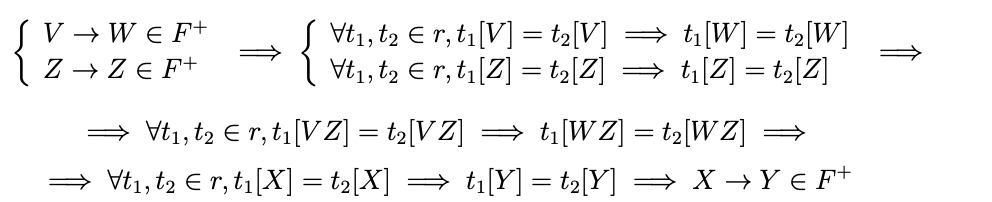
\includegraphics[width=0.8\textwidth,keepaspectratio]{{im/1}}
        \end{center}
        \end{figure}
      \item Se l'$(n + 1)$-esimo assioma applicato è l'assioma di transitività, allora è obbligatoriamente necessario che $\exists X \rightarrow Z, Z \rightarrow Y \in F^{A}$, ottenute con $k \leq n$ assiomi di Armstrong, affinché si abbia che:
      \begin{equation}
        X \rightarrow Z \in F^{A} \lor Z \rightarrow Y \in F^{A} \Rightarrow X \rightarrow Y \in F^{A}
      \end{equation}
      \pagebreak
      Siccome per ipotesi induttiva $X \rightarrow Z \in F^{A} \Rightarrow X \rightarrow Z \in F^{+}$ e $Z \rightarrow Y \in F^{A} \Rightarrow Z \rightarrow Y \in F^{+}$, si vede facilmente che:
      \begin{figure}[hbt]
        \begin{center}
            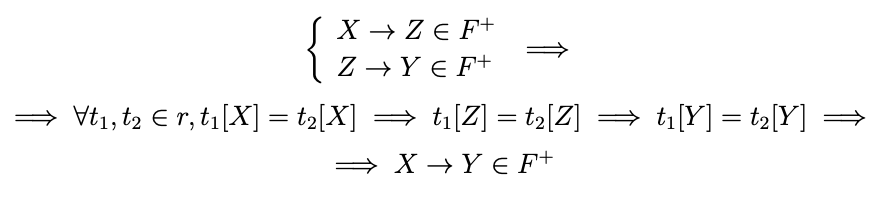
\includegraphics[width=0.7\textwidth,keepaspectratio]{{im/2}}
        \end{center}
        \end{figure}
  \end{enumerate}
\end{itemize}

\pagebreak
\subsection{Dimostrazione $F^{+} \subseteq F^{A}$}
\begin{figure}[hbt]
  \begin{center}
      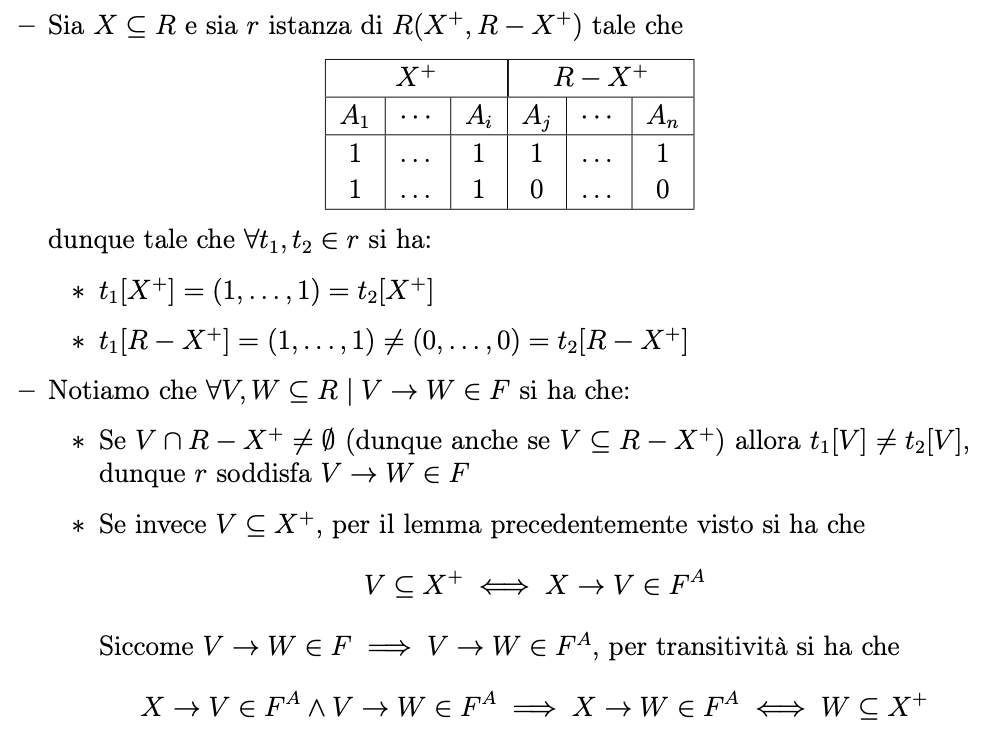
\includegraphics[width=0.75\textwidth,keepaspectratio]{{im/3}}
  \end{center}
  \end{figure}
  \begin{figure}[hbt]
    \begin{center}
        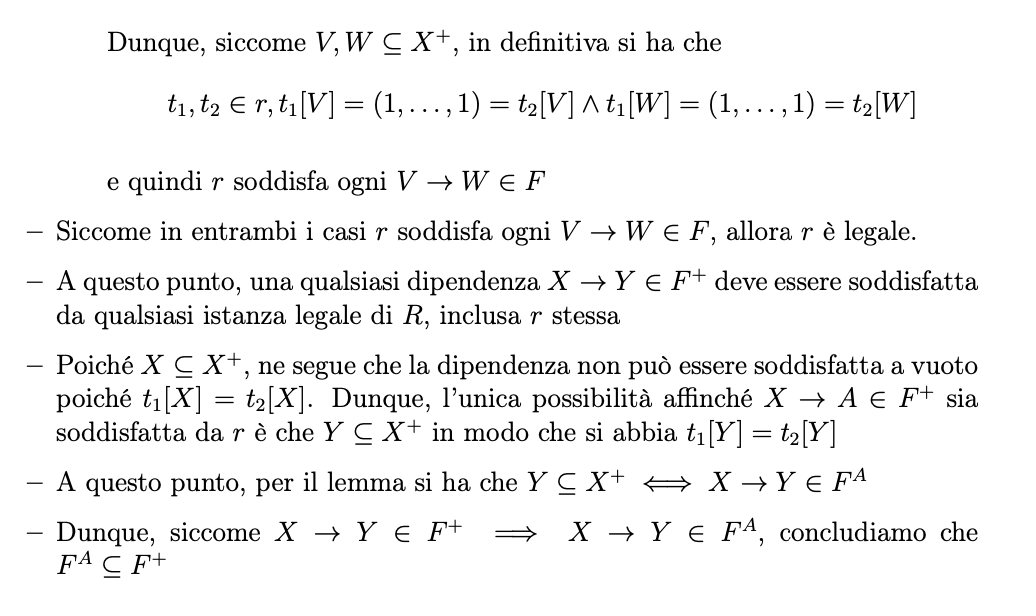
\includegraphics[width=0.8\textwidth,keepaspectratio]{{im/4}}
    \end{center}
    \end{figure}
    
    \begin{tcolorbox}[colback=white!20!white,colframe=green!70!black, title=Nota]
      Poiché $F^{+} = F^{A}$, per calcolare $F^{+}$ ci basta applicare gli assiomi di Armstrong sulle dipendenze in $F$ in modo da trovare $F^{A}$. \par Tuttavia, calcolare $F^{+} = F^{A}$ richiede tempo esponenziale, quindi $O(2^{nk})$: considerando anche solo l'assioma di riflessività, siccome ogni possibile sottoinsieme di $R$ genera una dipendenza e siccome i sottoinsiemi possibili di $R$ sono $2^{|R|}$, allora ne segue che $|F^{+}| >> 2^{|R|}$.
    \end{tcolorbox}

    




\pagebreak
\section{Chiusura di X}
\pagebreak
\section{Lemma Chiusura Inclusione}
\pagebreak
\section{Chiusura di X in G}
\pagebreak
\section{Join senza perdita}


\end{document}